\chapter{Arquitectura}
\label{chap:arquitectura}

\drop{E}{ste} capítulo pretende ofrecer una visión completa de la composición del sistema informático que constituye BreakBrain, profundizando en los diferentes componentes que lo forman y haciendo hincapié en los patrones de diseño utilizados y otros detalles de interés para el lector con conocimientos técnicos.

A lo largo de las siguientes secciones, se presentará la arquitectura detallada del sistema completo, para después estudiar a más bajo nivel los componentes principales por separado, centrando la atención en el del desarrollo de software.

\section{Composición del sistema}

\begin{figure}[h]
  \begin{center}
    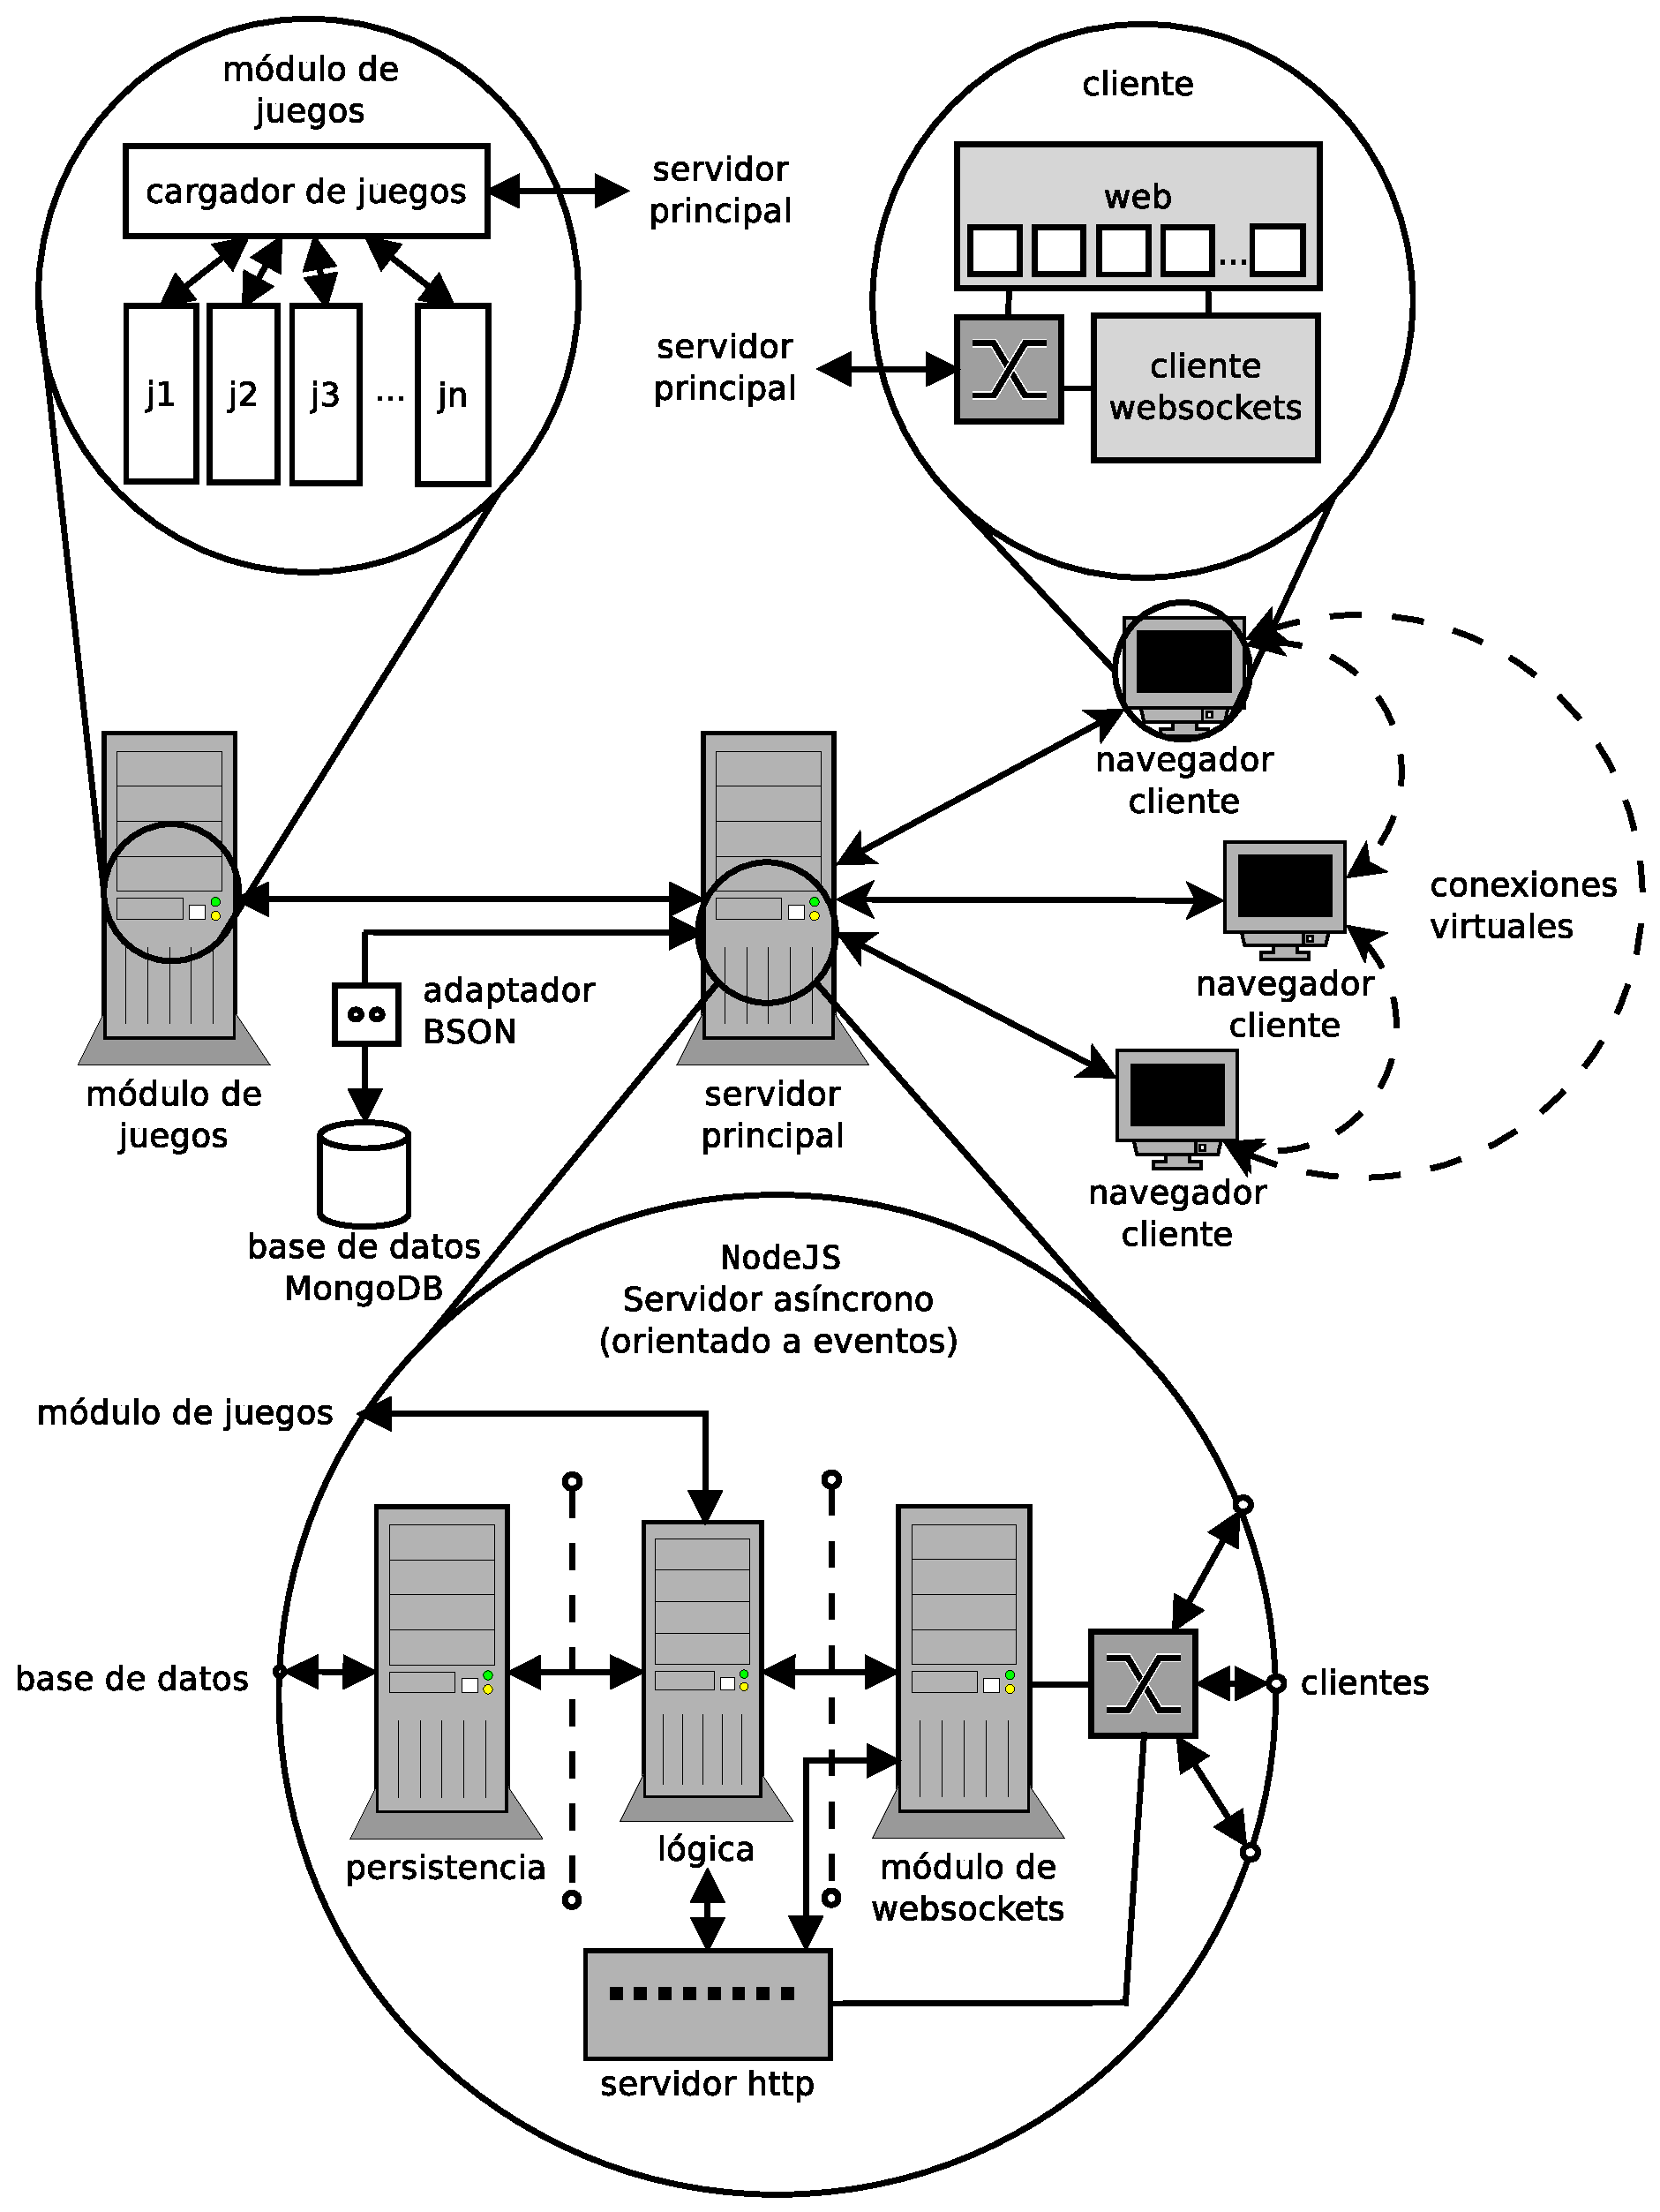
\includegraphics[width=\textwidth]{images/arquitectura.eps}
    \caption{Arquitectura detallada del sistema}
    \label{fig::arquitectura}
  \end{center}
\end{figure}

En la figura \ref{fig::arquitectura} se ofrece una visión detallada del los componentes que forman BreakBrain. Se trata de un enfoque de medio nivel que se adentra en la composición de los diferentes elementos de despliegue del sistema vistos en la sección \ref{sec::despliegue}. Como puede apreciarse, los dos protagonistas del enfoque {\it cliente-servidor} que sigue BreakBrain son tan complejos que se hace patente la necesidad de estudiarlos de forma detallada por separado.

A la vista de la figura \ref{fig::arquitectura} se perciben cuatro elementos esenciales en la composición del sistema:

\begin{itemize}
\item {\bf Cliente}\\Sitio web ejecutado sobre un navegador corriente. El uso de JavaScript que hace BreakBrain es intenso, tanto por la ejecución de los juegos como por el subsistema de comunicación permanente (necesario para los juegos multijugador), por lo que un navegador con buen soporte de JavaScript (como Chrome/Chromium \cite{chrome}) otorgará siempre una mejor experiencia de usuario.
\item {\bf Servidor principal}\\Se trata del corazón del sistema, compuesto principalmente por un servidor web corriente, al que se le ha añaido un servidor de comunicaciones mediante sockets TCP (con mensajes encapsulados en HTTP) para mantener una comunicación ininterrumpida con los clientes, y ofrecer así la base para la ejecución de juegos multijugador. El servidor se ejecuta en Nodester \cite{Nodester}, \acf{PAAS} de Software Libre que ofrece un buen servicio de forma totalmente gratuita.
\item {\bf Servidor de juegos}\\La piedra angular del servicio de juegos monojugador y multijugador. Construido de forma extensible, permite la integración de juegos de terceros en la plataforma. 
\item {\bf Sistema gestor de base de datos}\\Se ha optado por una base de datos no relacional MongoDB, alojada en los servicios de Amazon WS \cite{Amazon} y gestionada por MongoLab \cite{Mongolab}. Este último \acf{SAAS} se encarga del mantenimiento de la base de datos, asegurando la alta disponibilidad y escalabilidad.
\end{itemize}

\section{Arquitectura del sitio web}

La aplicación web de BreakBrain ha sido desarrollada utilizando NodeJS y ExpressJS, lo que fuerza la arquitectura de la misma hacia un enfoque \acf{MVC}. A su vez, la parte cliente (página web) ha sido desarrollada siguiendo este patrón.

\begin{figure}[H]
  \begin{center}
    \includegraphics[width=\textwidth]{images/mvc-cliente.png}
    \caption{Patrón MVC en el cliente de BreakBrain}
    \label{fig::mvc-cliente}
  \end{center}
\end{figure}

\subsection{Patrón MVC}

La arquitectura Modelo-Vista-Controlador en el cliente de la plataforma se distingue atendiendo a la división de los componentes que la constituyen en los siguientes tres grupos:

\begin{itemize}
\item {\bf Modelo}: Sistema de comunicación con el servidor.

\item {\bf Vista}: Interfaz gráfica con la que el usuario interactúa. Se trata de código \acs{HTML} embellecido con estilos \acs{CSS} y manipulado mediante JavaScript, haciendo uso de JQuery.

\item {\bf Controlador}: Lógica principal del cliente. Aquí pueden distinguirse dos componentes principales:

  \begin{itemize}
  \item Lógica de dominio a nivel de cliente
  \item Lógica de la parte cliente de los juegos
  \end{itemize}
\end{itemize}

En la figura \ref{fig::mvc-cliente} se aprecia el esquema expuesto.

\section{Arquitectura del servidor}

La aplicación web de BreakBrain ha sido desarrollada utilizando NodeJS y ExpressJS, lo que fuerza la arquitectura de la misma hacia un enfoque \acf{MVC}. A su vez, la parte del servidor ha sido desarrollada siguiendo este patrón.

\begin{figure}[H]
  \begin{center}
    \includegraphics[width=\textwidth]{images/mvc-servidor.png}
    \caption{Patrón MVC en el servidor de BreakBrain}
    \label{fig::mvc-servidor}
  \end{center}
\end{figure}

\subsection{Patrón MVC}

La arquitectura Modelo-Vista-Controlador en el servidor de la plataforma se distingue atendiendo a la división de los componentes que la constituyen en los siguientes tres grupos:

\begin{itemize}
\item {\bf Modelo}: Subsistema de persistencia, encargado de la manipulación de la base de datos.
\item {\bf Vista}: Interfaz de comunicación con el cliente mediante websockets.
\item {\bf Controlador}: Lógica central del servidor, compuesta por dos subsistemas:

  \begin{itemize}
  \item Lógica de dominio a nivel de servidor
  \item Lógica de servidor de los juegos
  \end{itemize}
\end{itemize}

En la figura \ref{fig::mvc-servidor} se aprecia el esquema expuesto.

\section{Diseño modular}

La propia esencia de NodeJS, la tecnología con la que BreakBrain ha sido implementado, guía al desarrollador hacia una estructura basada en módulos independientes.

\vspace{0.1cm}
\begin{figure}[H]
  \begin{center}
    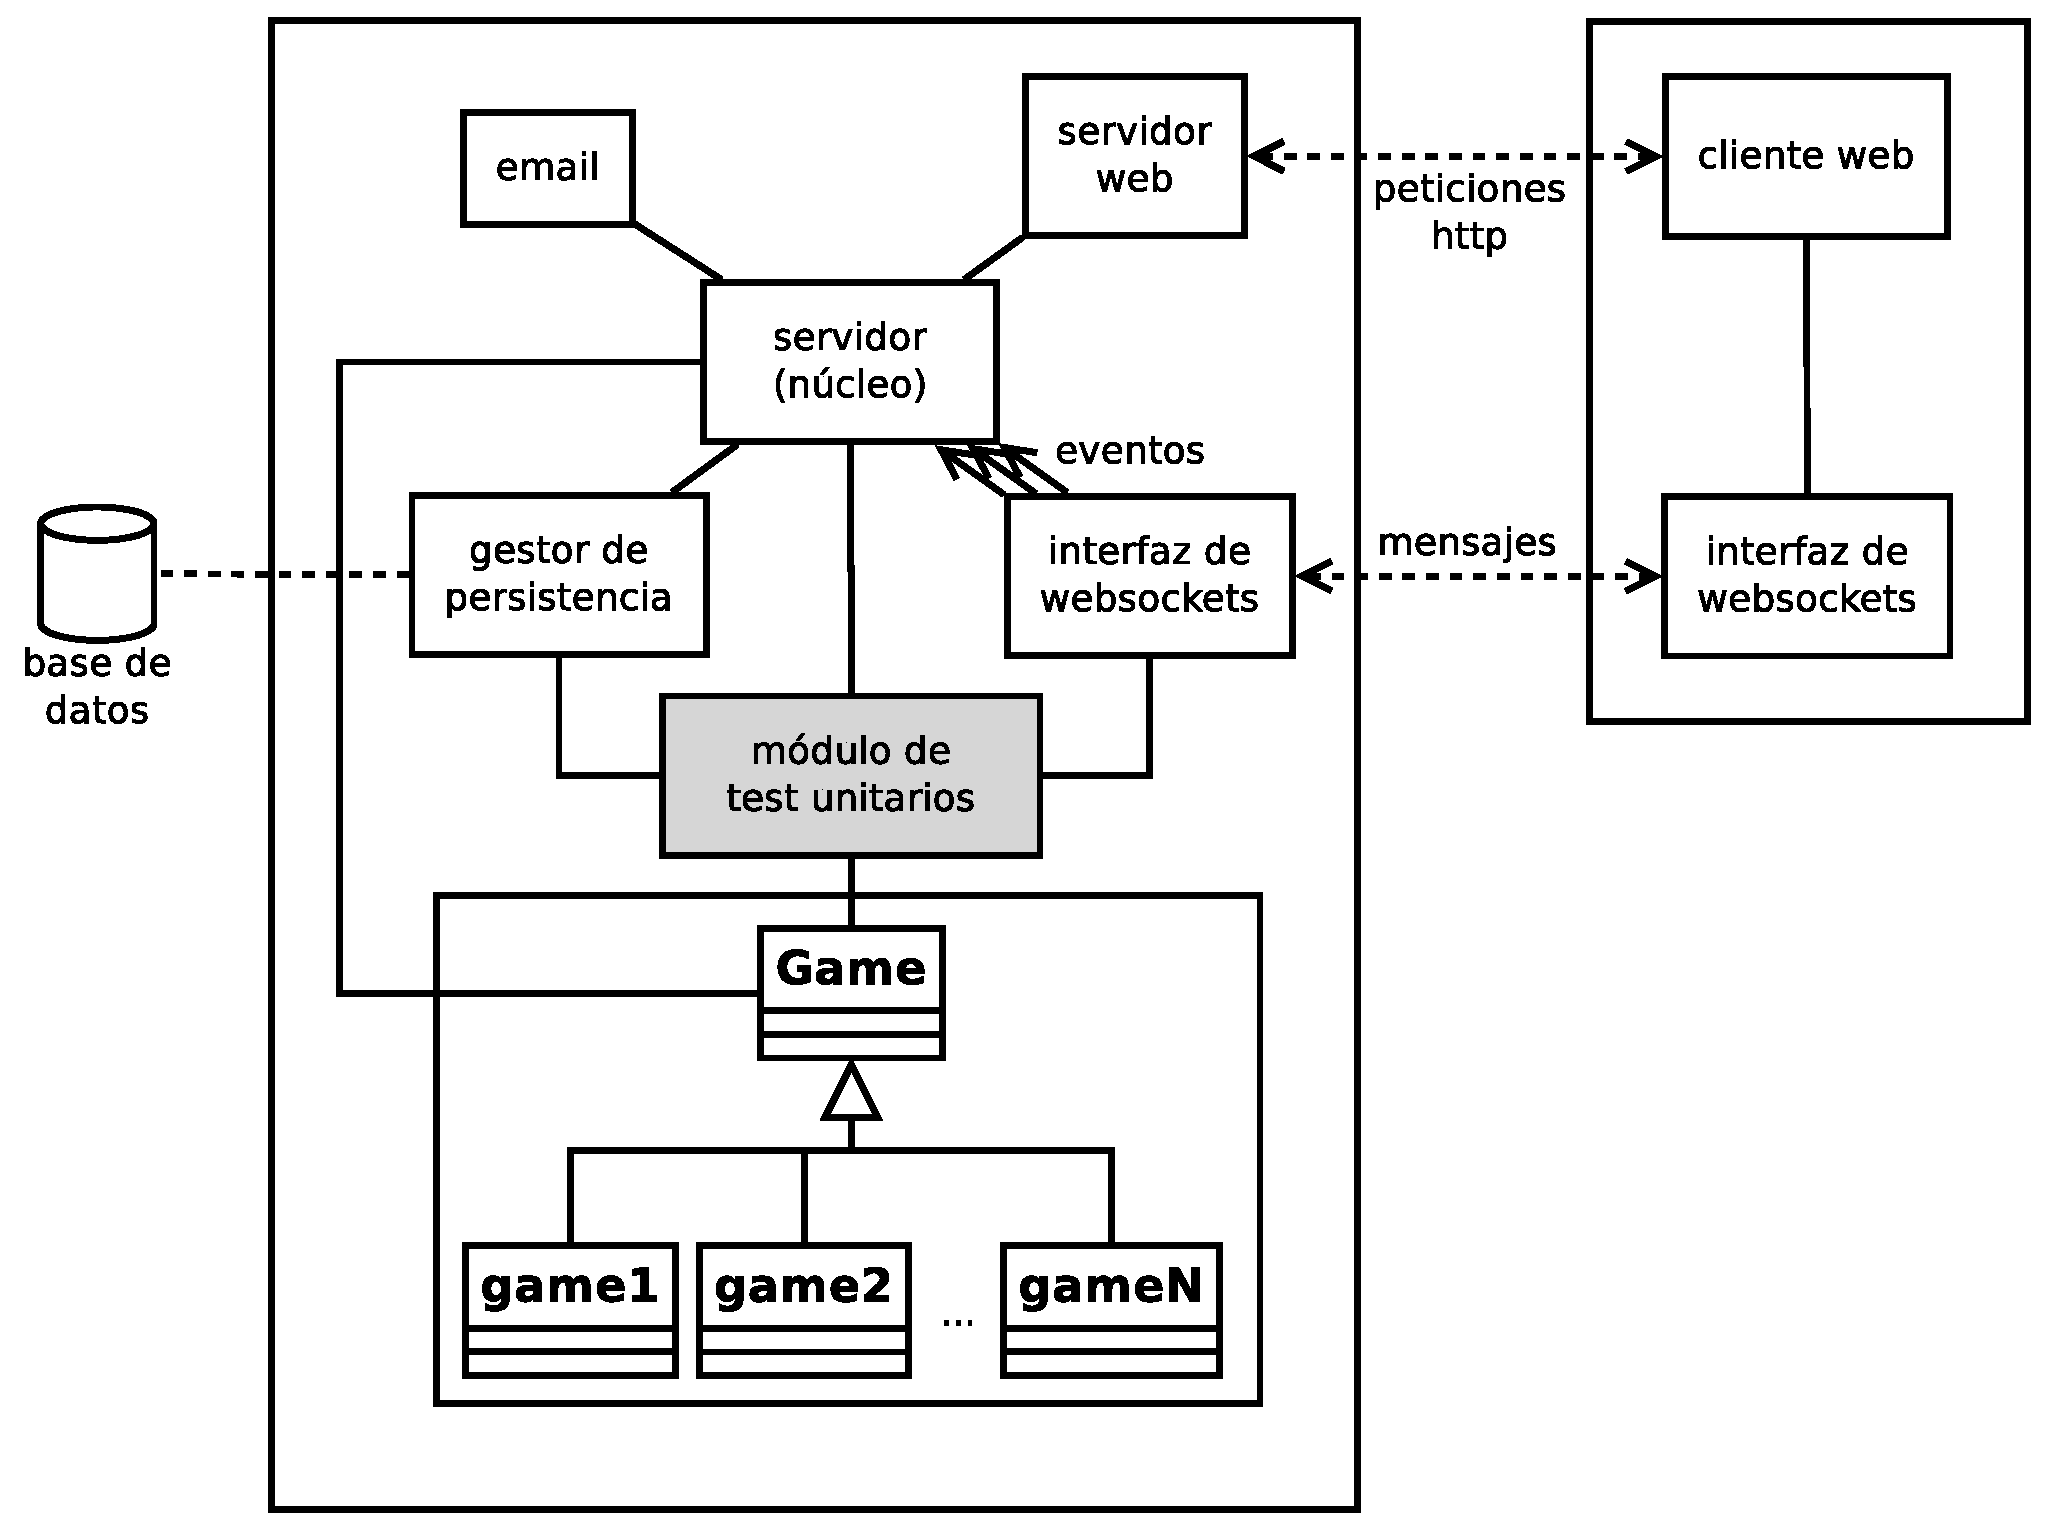
\includegraphics[width=\textwidth]{images/diseno.eps}
    \caption{Diseño modular del sistema}
    \label{fig::diseno}
  \end{center}
\end{figure}

En la figura \ref{fig::diseno} puede apreciarse la estructura modular de la plataforma, donde pueden distinguirse los siguientes componentes, agrupados según su funcionalidad:

\begin{itemize}
\item {\bf Gestor de persistencia}

Módulo encargado de la configuración y comunicación con el \acf{SGBD} utilizado (MongoDB).

\item {\bf Subsistema de email}

Módulo encargado del envío automático de emails.

\item {\bf Servidor web}

Módulo de manejo de peticiones y respuestas \acs{HTTP}, así como de la generación de contenido web dinámico para el cliente.

\item {\bf Servidor de websockets}

Módulo de conexión con el cliente mediante websockets. Mantiene (y pone a disposición de los juegos) una comunicación ininterrumpida con el navegador web de los usuarios.

\item {\bf Núcleo del servidor}

Módulo central, con la lógica de interconexión del resto de módulos y la creación de los propios servidores web y de websockets.

\item {\bf Módulo de test}

Módulo de pruebas de la plataforma.

\item {\bf Servidor de juegos}

Módulo encargado de la gestión de los juegos.

\item {\bf Cliente web}

El sitio web con el que el usuario interactúa.

\item {\bf Cliente de websockets}

Puente de comunicación entre el cliente y el servidor.

\end{itemize}




